% !TeX encoding = UTF-8
% !TeX spellcheck = de_DE

%% Dies gibt Warnungen aus, sollten veraltete LaTeX-Befehle verwendet werden
\RequirePackage[l2tabu, orthodox]{nag}

\documentclass[utf8,biblatex]{lni}
\bibliography{bibliographie}

%% Schöne Tabellen mittels \toprule, \midrule, \bottomrule
\usepackage{booktabs}

%% Zu Demonstrationszwecken
\usepackage[math]{blindtext}
\usepackage{mwe}

%% BibLaTeX-Sonderkonfiguration,
%% falls man schnell eine existierende Bibliographie wiederverwenden will, aber nicht die .bib-Datei händisch anpassen möchte.
%% Bitte \iffalse und \fi entfernen, dann ist diese Konfiguration aktiviert.

\iffalse
\AtEveryBibitem{%
  \ifentrytype{article}{%
  }{%
    \clearfield{doi}%
    \clearfield{issn}%
    \clearfield{url}%
    \clearfield{urldate}%
  }%
  \ifentrytype{inproceedings}{%
  }{%
    \clearfield{doi}%
    \clearfield{issn}%
    \clearfield{url}%
    \clearfield{urldate}%
  }%
}
\fi

\begin{document}
%%% Mehrere Autoren werden durch \and voneinander getrennt.
%%% Die Fußnote enthält die Adresse sowie eine E-Mail-Adresse.
%%% Das optionale Argument (sofern angegeben) wird für die Kopfzeile verwendet.
\title[Sicherheit in verteilten Systemen]{Sicherheit in verteilten Systemen}
%%%\subtitle{Untertitel / Subtitle} % falls benötigt
\author[Benita Dietrich \and Paul Finkbeiner]
{Benita Dietrich \footnote{DHBW Stuttgart Campus Horb, Florianstraße 15, 72160 Horb am Neckar, Deutschland} \and
 Paul Finkbeiner\footnote{DHBW Stuttgart Campus Horb, Florianstraße 15, 72160 Horb am Neckar, Deutschland}}
\startpage{1} % Beginn der Seitenzählung für diesen Beitrag
\editor{DHBW Stuttgart Campus Horb}    % Namen der Herausgeber
\booktitle{Sicherheit in verteilten Systemen} % Name des Tagungsband; optional Kurztitel
\year{2017}
%%%\lnidoi{18.18420/provided-by-editor-02} % Falls bekannt
\maketitle

\begin{abstract}
Abstract
\end{abstract}

\begin{keywords}
IT-Sicherheit, Verteilte Systeme, Software Engineering
\end{keywords}

\section{Einleitung}\label{Einleitung}

In der Vergangenheit kam es bei großen Unternehmen wie Facebook, Microsoft, Visa- und
MasterCard zum Teil mehrmals zu einer Entwendung von Kundendaten. Durch Attacken wie
Buffer Overflows, Viren oder andere Angriffsvektoren werden Maschinen und Benutzer auf
der ganzen Welt bedroht. Die Entwicklung des Internets legte ein besonderes Augenmerk auf
den Bereich der Netzwerksicherheit. Trotz vieler Bemühungen von IT-Sicherheitsexperten
und dem vorhanden sein leistungsfähiger Sicherheitsprotokolle und kryptografischen
Modulen kann ein vollständig sicheres System immer noch nicht gewährleistet werden.
Oftmals ist in dem Zusammenhang mit Daten Leaks nicht unbedingt die Kommunikation
zwischen Client und Server, sondern die eigentliche Software am Datenverlust maßgeblich
beteiligt. Die Gründe für das Schreiben unsicherer Software liegen oftmals an der mangelnden
Wahrnehmung von Fehlern seitens der Softwareentwickler oder der mangelnden
Verwendung von konkreten Mustern (Patterns) zur Lösung von Sicherheitsproblemen. In der
Software Entwicklung wird oftmals durch Frameworks bereits zur Entwicklungszeit die
Möglichkeit mitgeliefert bestimmte Sicherheitsmechanismen zu verwenden. Der Entwickler
hat die Aufgabe diese verstehen und richtig einsetzten zu können. Ein deutlicher Trend ist
momentan im Autonomisierungsbereich zu beobachten. Mit dem steigenden Einsatz von
Software in z.B. Haushaltsgeräten wird sich das Thema Sicherheit noch verschärfen. 
\newline
Im Rahmen der Projektarbeit wird die Frage beantwortet, wie
verteilte Systeme sicher gestaltet und implementiert werden können. 
Zunächst sollen die Begriffe Sicherheit und verteilte Systeme definiert werden, 
um einen ersten Einblick in das Thema zu bieten. 
Hinführen soll die Einführung auf die Beantwortung der Frage, 
was vor wem im System geschützt werden muss. Auf dieser Basis kann beschrieben werden, 
was es für Angriffe auf verteilte Systeme gibt. 
Welche Sicherheitslücken können von Angreifern ausgenutzt werden? 
Weiterhin sollen Anforderungen an verteilte Systeme abgeleitet und konkret definiert werden. 
Welche Sicherheitsdienste werden benötigt, um diese Anforderungen umzusetzen? 
Neben einer allgemeinen Definition dieser Dienste soll auch ein konkreter Vergleich mit der tatsächlichen Praxis erfolgen. 
Wie erfolgt die Sicherstellung eines sicheren Systems in der Praxis? 
Für den Vergleich kann ein Beispiel herangezogen werden. 
Um zu zeigen, dass das theoretisch erläuterte funktioniert, soll ein Prototyp entwickelt werden. 
Der Prototyp soll abstrakt einige Sicherheitsdienste implementieren und so das zuvor erklärte demonstrieren. 
Zur Umsetzung der Prototypen sollen geeignete Technologien und Architekturen gesucht und evaluiert werden, 
sodass der beste und einfachste Ansatz ausgewählt wird.


\subsection{Einführung in verteilte Systeme}\label{EinfuerungInVerteilteSysteme}

Für den Begriff \glqq verteilte Systeme \grqq{} liegt keine eindeutige Definition vor. Verschiedene Autoren definieren den Begriff der verteilten Systeme leicht unterschiedlich.
Nach A. Tanenbaum aus dem Jahre 2003 ist ein verteiltes System eine Menge voneinander unabhängiger Computer, die dem Benutzer wie ein einzelnes kohärentes System
erscheinen \citet{Mandl.2009}. Jeder Baustein kann seine Instanz auf unterschiedlichen oder aber auch auf dem gleichen Rechner haben. Die Systeme stellen je eigene Prozesse dar,
 die keinen gemeinsamen
Speicher haben und so autonom agieren können. Besonders wichtig ist die Koordinierung der Systeme und die Kommunikation zwischen ihnen.
\\\\
In den meisten Quellen wird unter dem Begriff verteiltes System ein verteiltes Anwendungsystem verstanden. Dies ist ein Softwaresystem, das das Prinzip der verteilten Systeme 
nutzt um ein 
Problem aus dem bereich der elektronischen Datenverarbeitung löst. Es gibt jedoch einige weitere Klassen von verteilten Systemen. Eine konkrete Einteilung ist noch nicht gegeben, sodass
mehrere Autoren unterschiedliche Klassifizierungsarten verfolgen. Die am häufigsten verwendete Klassifizierung ist die von A. Tanenbaum. Er unterteilt die verteilten Systeme
in drei Klassen ein. Zunächst nennt er die verteilten Computersysteme. Hierzu gehören Systeme wie Cloud- oder Grid-Computing. Dies sind jeweils Rechnersysteme die über LAN miteinander verbunden
sind und gemeinsam eine verteilte Anwendung unterstützen (vgl \citet{Mandl.2009}). Weiterhin nennt Tanenbaum verteilte Informationssysteme.
Informationssysteme dienen hauptsächlich der Regelung von betriebsinternen und -externen Prozessen, die dem Austausch von Informationen dienen \citet{Lackes.o.J.}
Hierunter werden auch die Anwendungsysteme eingeordnet. Als konkrete Beispiele lassen sich elektronische Bibliotheken oder Reisebuchungssysteme nennen.
Zuletzt gibt es verteilte pervasive Systeme. Hierunter werden kleine, batteriegetriebene oder auch mobile verteile Systeme eingeordnet (vgl \citet{Mandl.2009}).
\newline
Die verteilten Systeme schneiden neben der Informatik viele weiter Anwendungsdomänen an. Für das Finanz- und Vetriebswesen lassen sich eCommerce wie PayPal oder Ebay auflisten. 
Im Bereich Vertrieb und Logistik spielen heutzutage Navigationssysteme wie Google Maps eine große Rolle. Auch im Gesundheitswesen sind verteilte Systeme nicht mehr wegzudenken. Sie dienen unter
der Überwachung der Lebensfunktionalitäten von Patienten. Besonders in Zukunft werden verteilte Systeme für erneuerbare Energien, beispielsweise Windkraftwerke, außerordentlich wichtig sein. \citet{o.V.2011}
\\\\
Allgemein gibt es für verteilte Systeme jedoch einige Vorteile gegenüber herkömmlichen Systemen. Die Autonomie der Systeme bedingt eine verbesserte Ausfallsicherheit.
Fällt ein System aus, so sind die anderen hiervon nicht betroffen und können problemlos weiterarbeiten. 
Die Skalierbarkeit und Lastverteilung stellt einen weiteren Vorteil dar. Skalierbarkeit bedeutet dass die Last auf die einzelnen Komponenten verteilt, sodass kürzere Lade-und Antwortzeiten
erreicht werden. Größere rechenintensive Prozesse werden auf leistungsstarker Hardware ausgeführt, kleinere Prozesse auf schlechterer Hardware. Um das System zu ergänzen können problemlos weitere
Systeme oder Komponenten hinzugefügt werden. Die daraus erfolgende Flexibilität kommt der Anpassung an Anforderungen zu Gute. Das System kann nach Belieben geändert werden und auf Änderungen
in den Systemanforderungen schnell agieren. Zudem können Funktionalitäten des Systems auf mehrere Entwicklungsteams aufgeteilt werden. Jedes Team kann autonom voneinander arbeiten. Dies stellt
einen schnellen und effizienten Entwicklungsprozess sicher. Die entstehenden Teile hinter dem gesamten System kann dem Nutzer verborgen werden. Dies bezeichnet man als Verteilungstransparenz. So sieht der Nutzer
lediglich die Anwendung kennt aber keine genauen Hintergrundprozesse oder auftretende Fehler in einem Teilsystem. \citet{Mandl.2009}
\newline
Jedoch gibt es auch einige Nachteile die unter der Verwendung von verteilten Systemen auftreten können. Es können viele Abhängigkeiten zwischen Teilkomponenten entstehen, 
die sogar einem Single-Point-of-Failure entstehen lassen können. Unter einem SPOF versteht man eine Komponente, deren Ausfall den Ausfall des kompletten Systems mit sich zieht. Weiterhin kann
es zu Problemen in der Homogenität der Gesamtanwendung kommen. Dies entsteht durch Verwendung verschiedener Programmiersprachen oder unterschiedlichen Oberflächen Designs in den Teilsystemen. 
Weiterhin kann es zu Problemen in der Sicherheit kommen, die im nachfolgenden Abschnitt näher erläutert werden.

\subsection{Sicherheit}\label
In diesem Abschnitt wird genauer auf den Sachverhalt eingegangen welche Gefahren IT-Systemen drohen.
IT-Sicherheit ist ein Teil der Informationssicherheit und befasst sich mit der Planung, Maßnahmen und Kontrollen, die dem Schutz der IT dienen.
Sie reicht dabei vom Schutz einzelner Dateien bis hin zur Absicherung von Rechenzentren und Cloud-Diensten. 
Der Bereich von IT-Sicherheit ist grob in folgenden vier Teilbereiche einzugliedern: 

Quelle: https://www.security-insider.de/it-security-umfasst-die-sicherheit-der-ganzen-it-a-578480/

\paragraph{Schutz von Informationen und IT-Systemen}
Das auch als \glqq Endpoint Security \grqq{} bezeichnete Grundkonzept der IT-Sicherheit befasst sich mit dem durchführen 
Organisatorischer Maßnahmen die den unbefugten Zugriff auf Geräte verhindern soll. 
Die genaue Art der Geräte spielt dabei keine Rolle es kann sich um Notebooks, Tablets, PCs oder andere Geräte handeln. 
Geschützt werden die Endgeräte vor verschiedenen Arten von Schadsoftware oder vor unbefugten Systemzugriffen. 
Besonders durch trends in der Unternehmenskultur wie bspw. \glqq Bring your own device \grqq{}, gewinnt der Schutz der Firmeneigenen 
IT-Systeme immer mehr Bedeutung. 
Einige Maßnahmen haben sich im Bereich der Endgerätsicherheit heraus gezeichnet: 

\begin{itemize}
    \item Malware-Schutz
    \item Anwendungsisolation
    \item URL-Filter
    \item Client-Firewalls
\end{itemize}
\citet{Luber.2020}

Durch den umfassende Schutzmaßnahmen in diesem Bereich der IT-Sicherheit kann ein Großteil von Sicherheitsrisiken bereits 
verhindert werden. Ebenfalls ist durch den Schutz der Endgeräte durch Sicherheitsmechanismen wie Firewalls zusätzlich zu den 
Anwendungen auch das Betriebssystem des Gerätes geschützt. 

\paragraph{Schutz von Vernetzungen}
Netzwerkinfrastrukturen erstrecken sich heutzutage meistens über mehrere Geräte und Anwendungen hinaus. Der Schutz dieser 
Netzwerke wird allgemein auch als Netzwerksicherheit bezeichnet. Besonders im Zusammenhang mit verteilten Systemen muss auf diesem Punkt besonders Wert gelegt werden.
Es gilt die Systeme mit Verbindung ins Internet von Cyber-Bedrohungen abzuschirmen. Hierbei besteht das Ziel technische und organisatorische 
Maßnahmen so durchzuführen das die Integrität und Verfügbarkeit von Daten innerhalb eines Netzwerks und somit auch eines verteilten Systems stets gewährleistet werden. 
Innerhalb eines Netzwerkes hat sich eine Vielzahl an Techniken bereits etabliert. 
Zentraler Bestandteil für eine Sichere Kommunikation eines Netzwerks stellt dabei die Firewall dar. Firewalls kontrollieren den Datenfluss zwischen den 
Netzwerken, insbesondere zwischen dem Firmennetzwerk und dem Internet. Eine genauere Erläuterung der Schutzmaßnahmen und möglichen Angriffsvektoren im Zusammenhang mit 
der Vernetzung von mehreren Systemen wird zum späteren Zeitpunkt noch einmal genauer erläutert. 

Quelle: https://www.security-insider.de/was-bedeutet-netzwerksicherheit-a-578391/

\paragraph{Schutz des Benutzers}\label{Schutz_des_Benutzers}
Der Anwender selbst ist auch Bestandteil der IT-Sicherheit. Es muss von vorne herein festgelegt werden welcher Benutzer auf welches System zugreifen darf. 
Das Festlegen solcher Richtlinien wird als \glqq Identity- und Access Management \grqq{} bezeichnet und regelt die zentrale Verwaltung von Identitäten und Zugriffsrechten auf unterschiedlichen
Systemen und Applikationen. Für die Erteilung von Zugriffsrechten muss sich ein Benutzer Authentifizieren und Autorisieren. 
Die Authentifizierung ist der Prozess bei dem der Benutzer dem System mittels Benutzerdaten bestätigt, dass er derjenige ist, für den er sich ausgibt. Die Autorisierung 
wird anschließend durchgeführt um die Systeme und Ressourcen festzulegen auf die der Benutzer Zugriff erhält. Das Identity- und Access Management hat die 
Aufgabe für eine Vereinfachung und Automatisierung der Prozesse zu sorgen. 

\paragraph{Verhinderung von Schwachstellen}
Die meisten Bedrohungen in modernen IT-Systemen bestehen durch das Vorhandensein von Schwachstellen. Eine Aufgabe und ein Teilbereich der IT-Sicherheit sollte also auch 
das aufspüren und schließen von Sicherheitslücken sein. Oft treten solche Sicherheitslücken in Software auf, wenn ein Benutzer mehr machen kann als er eigentlich darf. 
Bei der eingesetzten Software muss durch Netzwerkadministratoren und Anwendungsbetreuer immer darauf geachtet werden, dass die Software immer auf dem aktuellesten Stand ist. 
\newline
Die Teilbereiche der IT-Sicherheit geben einen Eindruck welche Komponenten zu schützen sind. 
Die Quelle von Angriffen ist aber meistens noch wichtiger als das eigentliche Schutzziel. Aus diesem Grund wird eine genauere Betrachtung dahingehend 
erläutert, vor wem ein Schutz überhaupt notwendig ist. 
\newline
Das erste Bild das bei dem Gedanken eines Angreifers im IT-Umfeld entsteht, ist das Bild des Hackers. Allerdings sind diese meist nur ein Teil der Gefahren die auf IT-Systeme drohen. 
Auf IT-Systeme wirken die Naturgesetzte. Komponenten mit mechanischen Komponenten wie bspw. Festplatten oder Laufwerke sind besonders anfällig für Verschleiß. 
Ebenso wie die Wirkung der Naturgesetze stellen auch Naturkatastrophen eine Gefahr für IT-Systeme dar. In Firmen wird heutzutage bereits bei der Planung von 
IT-Infrastrukturen jede mögliche Eventualität bedacht und im Vorfeld auf Redundanz geachtet. Tritt so bspw. ein Feuer aus gibt es einen Rohrbruch oder eine Überschwemmung sollte 
eine Unterbrechungsfreie Redundanz der IT-Systeme weiterhin gewährleistet werden. 
\newline
Im Gegensatz zu natürlichen Ursachen kann auch der Mensch durch Unfähigkeit oder Nachlässigkeit eine Gefahr der IT-Sicherheit darstellen. 
Umso wichtiger ist es die Richtlinien für den Zugang an ein IT-System so granular wie möglich zu distanzieren \autoref{Schutz_des_Benutzers}.
\newline 
Auch andere IT-Systeme können die Sicherheit von verbundener IT-Systeme gefährden. Angenommen eine Person mit schlechter Intention versucht einen Zugang zu möglichst vielen 
IT-Systemen eines Netzwerks zu erlangen. Wenn es ihm gelingt eine Schwachstelle eines Systems zu erlangen erhält dieser die Möglichkeit trotz Firewallrichtlinien, einen Zugang 
auf alle weiteren Systeme zu erlangen, zu denen entsprechende Richtlinien in der Firewall festgelegt wurden. Dieses Verhalten wird heutzutage meist durch die Schadsoftwareart des 
\glqq Computerwurms \grqq{} realisiert. Nachdem dieser auf einem IT-System ausgeführt wurde hat es das Bestreben sich selbst, bspw. über das Netzwerk, zu vervielfältigen.

\section{Sicherheitslücken}\label{Sicherheitsluecken}
Damit ein verteiltes System möglichst sicher gestaltet werden kann, ist eine konkrete Analyse des Systems notwendig. Die Analsyse deckt Sicherheitslücken auf und evaluiert welche Angriffe auf welche Systemteile vorgenommen
werden könnten. Um hierfür näheres Verständnis zu erlangen, werden zunächst konkrete Angriffe auf verteilte Systeme definiert und daraus Anforderungen abgeleitet.

\subsection{Angriffe}

Informationstechnische Systeme werden heute kaum vollständig isoliert eingesetzt. Das beste Beispiel
dafür sind verteilte Systeme. Die Kommunikation zwischen den Systemen findet dabei über lokale und globale 
Netze statt. Dabei wird die globale Vernetzung oft von Tätern für schädliche Aktivitäten missbraucht.
Die Motivation hinter einer solchen Aktivität ist häufig Geld, Sabotage, Einflussnahme oder Informationsbeschaffung. 
Eine genaue Einteilung der Bedrohungen und der dazugehörigen Schutzziele für Systeme in der Informationstechnik sieht so aus:

\begin{tabular}[h]{l|c}
    Bedrohungen & Schutzziele \\
    \hline
    Unbefugter Informationsgewinn & Verlust der Vertraulichkeit \\
    Unbefugte Modifikation von Informationen & Verlust der Integrität \\
    Unbefugte Beeinträchtigung der Funktionalität & Verlust der Verfügbarkeit \\
\end{tabular}


Vertraulichkeit = Informationen werden nur Berechtigten bekannt.
\newline
Integrität = Informationen sind richtig, vollständig und aktuell
oder aber dies ist erkennbar nicht der Fall.
\newline
Verfügbarkeit = Informationen sind dort und dann zugänglich,
wo und wann sie von Berechtigten gebraucht werden.

Bei dem Aufbau eines verteilten Systems sollte stets darauf geachtet werden die Werte 
aufrecht zu erhalten. Eine genauere Beschreibung der Schutzziele wird in \autoref{Sicherheitsdienste} genannt. 
Zur Besseren Beurteilung und Abwehr von Angriffen teilt man diese in verschiedene Kategorien ein,
die jeweils ein Abweichen vom normalen Datenfluss anzeigen.

\begin{figure}
    \centering
    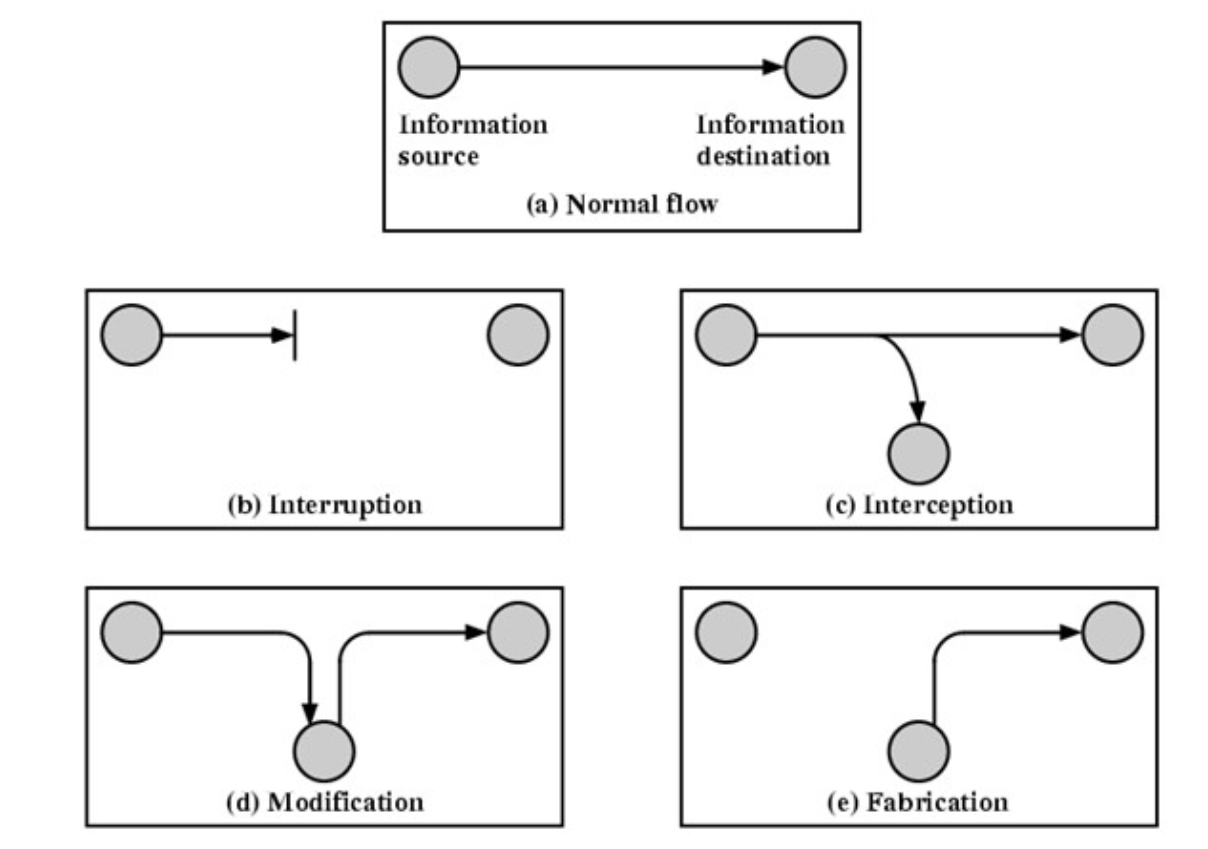
\includegraphics[width=\textwidth]{images/angriffe_pic1.png}
    \caption[Beschreibung für Inhaltsverzeichnis]{Bildbeschreibung} 
    \label{Referenz}
\end{figure} 

\paragraph{Unterbrechungen}
Von einer Unterbrechung wird immer dann gesprochen wenn ein Bestandteil des 
IT-Systems zerstört oder unbrauchbar gemacht wird. Die Angriffe zielen darauf 
ab die Verfügbarkeit des betroffenen IT-Systems zu schwächen. 

\paragraph{Abfangen}
Die oft als \glqq Man-in-the-middle \grqq{} Angriffe bezeichneten Attacken sind dieser 
Kategorie zuzuweisen. Ein nicht berechtigter Benutzer versucht die Vertraulichkeit des 
IT-Systems zu kompromittieren.  

\paragraph{Modifikation}
Von einer Modifikation spricht man immer dann wenn ein Angreifer Zugriff auf einen 
Systemteil gewinnt und auf diesem Daten manipuliert. Diese Angriffsart zielt 
darauf ab die Integrität der Daten zu gefährden. 

\paragraph{Fälschung}
Wenn ein Dritter gefälschte Objekte in eine System einschläust spricht man von 
einer Fälschung. Die Fälschung kompromittiert die Authentizität der Daten. 
Ein Beispiel hierfür wäre sogar bereits die Urkundenfälschung auf einem Computersystem. 

Bei der folgenden Betrachtung von Angriffen auf verteilte Systeme werden die Angriffe jeweils einer 
der aufgeführten Kategorien zugeordnet. 

Der bisher wohl bekannteste Cyber-Angriff wurde 2017 in Form der Ransomeware \glqq WannaCry \grqq{} bekannt.
Mithilfe einer Schwachstelle konnte eine Hackergruppe einen sog. Kryptotrojaner über das Netzwerk
auf sehr viele IT-Systeme verteilen. Besonders interessant in dem Zusammenhang mit verteilten Systemen ist 
das Vorgehen des Trojaners in Unternehmen und Institutionen wir bspw. Krankenhäusern. 
In einigen Krankenhäusern wurden alle Geräte, einschließlich Medizinisches Equipment von 
der Schadsoftware verschlüsselt. 
Die Art der Implementierung des Exploits unterschied sich insofern von anderen Verschlüsselungsprogrammen, 
dass der Benutzer keinen Fehler machen musste um betroffen zu sein. 
Der Virus wurde weder durch einen Word Macro, noch einen verdächtigen Link auf den Computer übertragen. 
Besonders bei großen Unternehmen ohne die nötigen Sicherheitsmaßnahmen wurde großer Schaden angerichtet. 
Teilweise musste bei solchen Fällen die Produktion gestoppt werden, was zu einem enormen wirtschaftlichen 
Schaden geführt hat. 
Ein Solcher Angriff zielt auf die Kompromittierung der Verfügbarkeit und Integrität der Daten des 
Zielsystems ab und sorgt somit für eine Unterbrechung- und Modifikation des normalen Datenflusses. 
\\\\
Ein ebenfalls sehr bekanntes Beispiel für einen Cyber-Angriff ist die Malware \glqq Stuxnet. \grqq{}
Das Ziel des Angriffs war es die Leittechnik zur Urananreicherung im Iran außer Kraft zu setzen. 
Dem Wurm war es möglich, sich über USB-Sticks unbemerkt sogar auf Computersysteme ohne Internetzugang 
auszubreiten. Gerieht die Schadsoftware auf einen Rechner der mit einer bestimmten Maschinensteuerung 
verbunden war, programmierte er diese automatisiert um. Das primäre Ziel des Computervirus bestand darin 
die Verfügbarkeit des Zielsystemes zu kompromittieren was zu einer Unterbrechung des normalen Datenflusses führte. 
\\\\
Die Gefahren von Cyberattacken sind sehr umfangreich die hohe Komplexität der Schadsoftware ist der 
Grund warum man nie von einem vollständigig sicheren System sprechen kann. 
Von dem Bundesamt für Sicherheit in der Informationstechnik (BSI) sind einige Interessante Fakten darüber veröffentlicht worden: 
\begin{itemize}
    \item Etwa alle zwei Sekunden erscheint ein neues Schadprogramm bzw. eine neue Variante
    \item Pro Minute werden ca. 2 digitale Identitäten in Deutschland gestohlen
    \item Pro Tag werden etwa 4-5 geziehlte Trojaner im Regierungsnetz entdeckt
    \item Pro Monat werden etwa 40.000 Zugriffsversuche aus dem Regierungsnetz auf schädliche Websiten blockiert
\end{itemize}


\subsection{Anforderungen an verteilte Systeme}
Um die Sicherheit im verteilten System gegen die möglichen Angriffe zu schützen müssen einige Anforderungen erfüllt werden. In diesem Abschnitt sollen
konkret die Sicherheitsanforderungen an die verteilten Systeme näher betrachtet werden. Um ein verteiltes System möglich sicher zu gestalten muss eine konkrete Sicherheitsanalyse vorgenommen werden. Hierbei werden alle möglichen Sicherheitslücken und Angriffspunkte aufgedeckt. 
Entsprechend müssen Lösungen und Sicherheitsmechanismen erarbietet und implementiert werden. Da die konkreten Anforderungen an ein verteiltes System sehr unterschiedlich sind und von der konkreten Art des Systems abhängt, werden hier nur einige konkrete Beispiele genannt.
\\\\
Zunächst ist es wichtig, dass das System die Daten der Benutzer vor Angreifern schützt, um Missbrauch zu verhindern. Hierzu zählen beim Beispiel Onlineshops Anmelde- oder Kontodaten. Die Daten und deren Übertragung
schützt ein Zertifikat.
\newline
Weiterhin müssen die Daten des Systems entsprechend ihrer Klassifizierung (öffentlich oder privat) verfügbar gemacht werden. Alle Benutzer werden passend autorisiert und erhalten Zugang zu den ihnen zugänglichen Informationen. Besonders sicher und gut autorisiert müssen dabei die Administratoren werden.
Bei einem Windkraftwerksystem soll beispielsweise nur der Instandhalter und der Manager Zugriff auf das gesamte System bekommen. Alle anderen Arbeiter erhalten nur Zugriff zu dem Teilsystem, welches sie für ihre Arbeit benötigen.
 Änderungen die die Benutzer vornehmen
werden getracked und nachvollziehbar dokumentiert. Auch ein Monitoring über die Systeme muss erfolgen, sodass ein Ausfall schnell erkannt und ein möglicher Unterbrechungs-Angriff verhindert werden kann.
Allgemein muss die Oberfläche so sicher wie möglich gestaltet werden. Weiterleitungen auf andere Seiten und Dienste sollten sicher sein, ebenso muss der Kunde vor Maleware die über das System
übertragen werden kann geschützt werden.
Weiterhin ist neben dem Schutz der Daten auch die Sicherheit der Kommunikation zwischen der Software und dem Kunde wichtig. Dies betrifft zum Beispiel das Senden von E-Mails an den Benutzer. Die Daten werden oft ungescihert
oder unvalidiert versendet. 
Zur Vermeidung von Fälschungen in der Datenhaltung muss das System gewissen Verschlüsselungsmechanismen bereitstellen. 
\citet{Kriha.2008}

\section{Sicherheitsdienste}\label{Sicherheitsdienste}

In den vorherigen Kapiteln wurden Angriffsmöglichkeiten und die Anforderungen an ein verteiltes System untersucht. In diesem Kapitel erfolgt eine Konkretisierung der Sicherheitsdienste, die
ein verteiltes System bereitstellen muss um als sicher zu gelten. Dieses Kapitel erklärt die unterschiedlichen Dienste und stellt sie anschaulich anhand von Beispielen dar.

\subsection{Vertraulichkeit}
Die Vertraulichkeit macht Daten nur für eine Gruppe von autorisierten Benutzern verfügbar und schützt sie so vor unbefugten Zugängen. Diese Daten können verschiedene Arten von Informationen,
wie zum Besipiel Nachrichten, Videos oder Filme, Passwörter oder Kontodaten sein. Ein konkretes Beispiel wäre ein Film auf Amazon Prime. Dieser Film ist nur denjenigen
Benutzern verfügbar, die ihn gekauft oder geliehen haben. Um ein weiteres Beispiel handelt es sich bei den Anmeldedaten eines Benutzers. Die Verbindung zwischen Benutzer
und Server muss stets verschlüsselt sein, sodass kein Unbefugter die Anmeldedaten abgreifen kann. \citet{Kriha.2008}
\\\\
In verteilten Systemen funktioniert der Vertraulichkeitsdienst  entweder durch Zugriffsbeschränkungen über einen Kontrollmechanismus oder Verschlüsselung der Informationen (vgl \citet{Mirhakkak.1993}).
Für die Verschlüsselung kann beispielsweise das TLSP Protokoll herangezogen werden. Die Informationen werden vom Protokoll vor dem Senden verschlüsselt und vor dem Empfang wieder entschlüsselt.
So werden die Nachrichten gesichert übermittelt, sind aber dennoch für die Kommunikationspartner zugänglich. Die Vertraulichkeit dient der Sicherstellung des Schutzes der Daten und stellt eine Grundvoraussetzung für erfolgreiche Authentifizierung
und Autorisierung dar. Der Vertraulichkeitsdienst stellt sicher, dass während dem Informationsaustausch keine Manipulationen oder Abfangen der Daten von passiven Angreifern erfolgt ist. \citet{Mirhakkak.1993}
Die Vertraulichkeit dient jedoch nicht nur dem Schutz der Daten vor Unbefugten, sondern trägt auch zur Anonymität der Benutzer bei.
In einem verteilten Informationssytem kann der Vertraulichkeitsdienst Beispielsweise durch Nutzerprofile erfolgen. Hier erhält jeder nur Zugriff auf die ihm zugewiesenen Bereiche. Die persönlichen Daten wie Name und
Adresse sind durch Anmeldename und Kennwort geschützt. Um zu verhindern, dass ein Unbefugter Anmeldename und Passwort abgreifen kann, wird die Verbindung mit einem Sicherheitszertifikat verschlüsselt.


\subsection{Authentifizierung}

Authentifizierung sorgt dafür, dass ein Benutzer gegenüber einem System verifiziert werden kann.
Der Begriff der Authentifizierung wird oft synonym mit den Begriffen Authentisierung und Autorisierung verwendet. 
Die Authentifizierung lässt sich in weitere Bestandteile untergliedern. Der erste Bestandteil ist die Authentisierung, 
wobei der Benutzer gegenüber dem System eine Identität vorgibt, die von diesem bestätigt werden soll. 
Auf die Authentisierung folgt anschließend die Authentifizierung. Bei dem Authentifizierungsvorgang werden die vom Nutzer 
eingegebenen Daten, also seine angegebene Identität, überprüft. Ist die Überprüfung abgeschlossen folgt die 
Autorisierung. Die Autorisierung ist für die Zuteilung der Zugriffsrechte verantwortlich. 
Durch den Prozess der Authentifizierung wird eine Identität an ein Subjekt/ Entität gebunden. 
Das Binden der Identität berechtigt den Benutzer bestimmte Dienste in Anspruch nehmen zu können. 
\newline
Es gibt verschiedene Arten wie eine Authentifizierung durchgeführt werden kann:
\begin{figure}
    \centering
    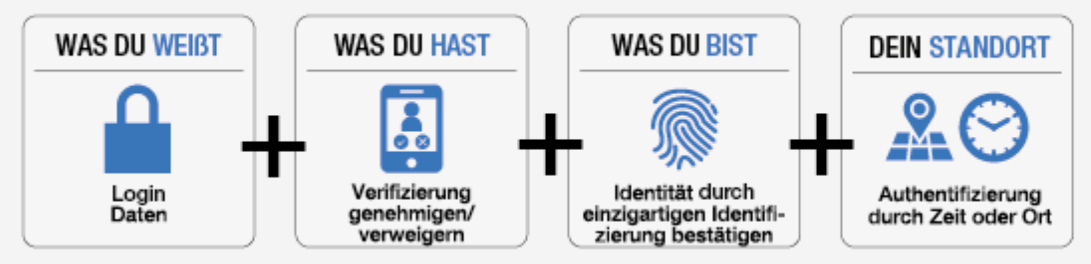
\includegraphics[width=\textwidth]{images/authent_pos1.png}
    \caption[Authentifizierungsarten]{Authentifizierungsarten} 
    \label{Authentifizierungsarten}
\end{figure} 

Im Zusammenhang mit verteilten Systemen im Internet ist die Authentifizierung durch Wissen,
also Benutzername und Passwort, weit verbreitet. 
Das Passwort besteht dabei meistens aus einer Zeichenkombination und wird über einen geschützten Kanal ausgetauscht. 
Besonders bei Diensten im Internet bietet sich die Verwendung von Hyper-Text-Transfer-Protocol-Secure (HTTPS), statt
des ungesicherten Hyper-Text-Transfer-Protocol (HTTP) an.
Das auslesen der Benutzerdaten aus dem Netzwerkverkehr ist so nicht mehr möglich. 
Mit Verwendung eines sicheren Protokolles für die Übermittlung der Daten ist die Übertragung zwischen den Systemen 
als Angriffsvektor ausgeschlossen. 
Sind die Daten erfolgreich und sicher an das Serversystem übermittelt worden müssen diese in bestimmter Form 
(bspw. in einer Datenbank) persistiert werden. 
Das festhalten der Daten im Klartext würde die Datenbank zu einem sehr lohnenden Ziel machen, da die Daten 
an einer stelle gesammelt einsehbar wären. 
Aus diesem Grund benutzt man verschiedene Verschlüsselungsfunktionen um zumindest die Passwörter in eine Form zu bringen,
die nicht wieder re-konstruiert werden kann. Das Anwenden der Verschlüsselungsfunktion wird 
als Hashing bezeichnet. Gehashte Passwörter in der Datenbank bieten eine notwendige Sicherheit um die Daten in sicherer Form 
dauerhaft zu abzulegen. Abgesehen von der Authentifizierung durch Wissen mittels Benutzername und Passwort gibt es die Möglichkeit sich durch 
Besitzt, Identität oder den Standort zu Authentifizieren. 
Besonders interessant für zusätzliche Sicherheit auf Client-Seite können die 
Authentifizierungsmöglichkeiten kombiniert werden. Die Kombination von bspw. einer Authentifizierung durch Wissen und von Besitz 
wird als 2-Faktor-Authentifizierung bezeichnet. Gelangt ein Angreifer an ein Passwort hat er so ohne die entpsrechende zweite 
Authentifizierungsmethode keine Möglichkeit die Identität des Benutzers anzunehmen. 

\subsection{Integrität}

Das Schutzziel Integrität umfasst sowohl die Korrektheit der Daten (Datenintegrität) 
als auch die korrekte Funktionsweise des Systems (Systemintegrität). 
Es gibt schwache und starke Integrität. 
Eine starke Integrität liegt vor, wenn keine Möglichkeit der unbefugten Datenmanipulation besteht. 
Von einer schwachen Integrität spricht man hingegen dann, falls eine Datenmanipulation zwar generell, 
aber auf keinen Fall unbemerkt möglich ist. 
Mögliche Manipulationen sind z.B. das
Verändern von Daten
Löschen von Daten
Einfügen von Daten
Grundsätzlich ist es fast unmöglich Veränderungen an digitalen Daten vollständig zu vermeiden. 
Dadurch das man die Veränderungen von Daten nicht vermeiden kann, versucht man dem Benutzer die 
Änderung der Daten erkennbar zu machen. 
Besonders im Linux Umfeld hat sich eine überprüfung von Downloads mittels Prüfsummen etabliert.
Zu der eigentlichen Download Dateien ist zusätzlich die Information \glqq SHA265SUM\grqq{ } gegeben (siehe \autoref{Pruefsumme}).
\newline
Es gibt verschiedene Arten wie eine Authentifizierung durchgeführt werden kann:
\begin{figure}
    \centering
    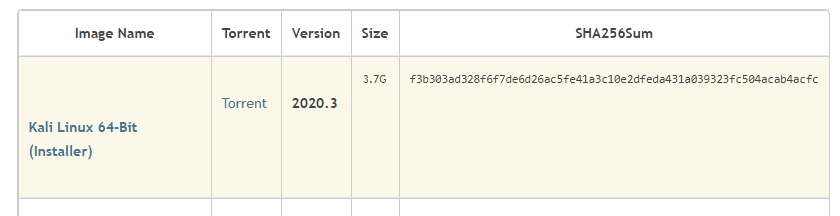
\includegraphics[width=\textwidth]{images/checksum_pic1.png}
    \caption[Prüfsumme]{Pruefsumme} 
    \label{Pruefsumme}
\end{figure}  
Nach dem Download der Datei kann die Prüfsumme über die heruntergeladene Datei erfolgen,
sind die beiden Hashwerte identisch ist der Download valide. 
Stimmen die beiden Prüfsummen nicht über ein, wurde der Download manipuliert und die 
Integrität der Daten wurde verletzt.

\subsection{Nicht-Anfechtbarkeit}

Das Schutzziel der Nicht-Anfechtbarkeit wurde früher hauptäschlich im Bereich des Informationsaustausches verwendet. Jedem Kommunikationsteilnehmer soll nachgewiesen werden können, welche Informationen er 
versendet oder erhalten hat. Hierfür werden verschiedene Arten der Nachweisbarkeit benötigt. Durch die Nachweisbarkeit der Identität wird das Verleugnen von Nachrichten verhindert und zusätzlich der Betrug verhindert.
Die Nachweisbarkeit des Sendens bezeugt, dass die entsprechenden Informationen auch wirklich gesendet wurden. Ergänzend hierzu kann die Nachweisbarkeit des Zustellens bezeugen, dass der Empfänger die Informationen
auch tatsächlich erhalten hat. \citet{Bedner.2010}
\\\\
Mit dem Zeitalter der Digitalisierung erweiterte sich diese Begriffdefinition auf Handlungen und Transaktionen (vgl \citet{Bedner.2010}).
Unter Nicht-Anfechtbarkeit versteht man heute das Erzeugen eines Nachweises für eine bestimmte Handlung oder Aktion. Der Beweis dient dazu, zu dokumentieren und festzuhalten was ein Benutzer getätigt hat. 
Der Nicht-Anfechtbarkeitsdienst
dient im Streitfall dazu, die erfolgten Aktionen zwischen zwei Kommunikationspartnern Dritten zu beweisen.
Ein konrektes Beispiel wäre ein Überwachungssystem mit Kameras und audiovisueller Aufnahme, wie es Kriha in seinem Buch \citet{Kriha.2008} beschriebt. Um die Daten vor Gericht verwertbar zu machen, muss garantiert werden, dass die Aufnahme von einer der Überwachungskameras stammt.
Weiterhin darf es nciht möglich sein Audiodateien einzuschleusen und so Daten zu fälschen. Auch in Online-Shops in Beriechen des E-Commerce ist Nicht-Anfechtbarkeit wichtig.
Kauft ein Kunde etwas, so muss der Shop genau festhalten was der Kunde gekauft hat. Sind diese Daten nicht-anfechtbar abgespeichert, so kann dem Kunde stets die Inanspruchnahme des zahlungspflichtigen Dienstes
bewiesen werden. Besonders wichtig ist auch wie beim Beispiel des Überwachungssystems die Glaubhaftigkeit des Nachweises, sodass die Möglichkeit der Fälschung von Nachweisen ausgeschlossen werden kann.
Der Nicht-Anfechtbarkeitsdienst sollte aus diesem Grund einen erfolgten Informationsaustausch so dokumentieren, dass der Nachweis nicht gefälscht oder selbst erzeugt sein könnte. 
den Begriff Nicht-Anfechtbarkeit verwendet man auch häufig zusammen mit dem Begriff \glqq Digitale Signatur\grqq{}. Auch die digitale Signatur ist eine Form der Garantie von Nicht-Anfechtbarkeit. 
Es wird die Identität des Benutzers überprüft und ein gültiges Dokument durch eine elektronsiche Unterschrift rechtskräftig unterzeichnet.
\\\\
Es gibt keine konkreten Algorithmen oder Vorgaben, wie der Nicht-Anfechtbarkeitsdienst in verteilten Systemen implementiert werden kann.
Die Implementierung ist stark von der Klasse des verteilten Systems abhängig.

\subsection{Zugriffssteuerung/Autorisierung}

Nachdem ein sicherer Tunnel durch die Dienste Authentifizierung, Vertraulichkeit und 
Integritätsschutz aufgebaut wurde, befasst sich die Autorisierung mit der Frage wie die Daten 
anschließend verarbeitet werden. 
In Computernetzwerken sowie im Bereich von verteilten Systemen bezeichnet die Autorisierung das Zuweisen 
und die Überprüfung von Zugriffsrechten. Damit bilden Autorisierung und Zugriffssteuerung eine Einheit und 
verantworten die Vergabe von Freigaben an den Benutzer. 
Es gibt verschiedene Arten wie festgelegt werden kann auf welche Ressourcen welcher Benutzer einen Zugriff hat. 
Meist werden die Benutzer zum Stand der Registrierung bereits in eine Benutzergruppe eingeteilt. 
Mithilfe von Gruppenbasierter Zugriffssteuerung können mehrere Rechte mit einem Mal an einen Benutzer übergeben werden. 
Zusätzlich kann mehr Arbeit in die Ganularität der Gruppenberechtigungen investiert werden, als 
wenn für jeden Benutzer eigene Rehte vergeben werden würden. 
Ein Besipiel für eine Gruppenbasierte Zugriffssteuerung ist die Rechtevergabe in Betriebssystemen wie Linux und Windows.
Bei Linux gibt es eine sog. \glqq root\grqq{}-Gruppe, die über Adminsitratorrechte verfügt. Ist ein Benutzerkonto teil dieser Gruppe
kann ohne Einschränkung Software Installiert werden. Ist ein Benutzer in keiner Gruppe muss für die Installation von Software 
das Administrator Kennwort eingegeben werden. 
In verteilten Systemen ist ein ähnliches Prinzip zu beobachten. So gibt es für eine Webanwendung oftmals 
eine Administratorgruppe und Beispielsweise eine Gruppe mit der Bezeichnung \glqq Kunde\grqq{} die nur den Zugriff auf 
einen Teilbereich der Webanwendung zulässt. 

\subsection{Verfügbarkeit}

Der Sicherheitsdienst Verfügbarkeit garantiert, dass das verteilte System und die angeforderten Daten für seine Benutzer zeitgerecht zur Verfügung steht. Die Datenverarbeitung muss stets ordnungsgemäß
und inhaltlich korrekt sein. \citet{Bedner.2010}
Dieser Dienst wird in den aufgeführten Quellen stets im Rahmen der informationstechnischen Systeme verwendet. Der Verfügbarkeitsdienst
  zielt vorallem darauf ab zu verhindern, 
dass Angreifer über Malware das System ausschalten. Oftmals funktioniert das Auschalten über mehrere kontaminierte Clients, die gleichzeitig auf das System zugreifen. 
Diese Aktion hat eine Überlastung des Ziel-Servers und infolgedessen einen System-Absturz zur Folge. \citet{Kriha.2008}
\newline
Betrachtet man die Dauer der Verfügbarkeit des verteilten Systems im Verhältnis zu der Gesamtzeit, so ist das verteilte System optimalerweise 100\% verfügbar. Dies kann in der Realtiät jedoch kaum erreicht werden.
Fällt ein System aus, so wird die gesamte Ausfallzeit als Downtime bezeichnet. \citet{Bedner.2010}
\newline
 Um die Downtime des Systems möglichst gering zu halten gibt es verschiedene Maßnahmen, die je nach Art des verteilten Systems und auch
dem konkreten Grund des Ausfalls variieren. Als eine allgemeine Maßnahme nennt beispielsweise Bedner in seinem Zeitungsartikel \citet{Bedner.2010} die Verwendung redundanter Systeme. Bei einem Ausfall
des Hauptsystems kann das redundante System verwendet werden und ein Absturz wird somit verhidndert. Dies betrifft beispielsweise besonders verteilte Systeme der erneuerbaren Engerien.
Für das konkrete Beispiel eines informationstechnischen Systems schreibt Kriha in seinem Buch \citet{Kriha.2008} über das Besipiel eines Angriffs. Um zu verhindern das kontaminierte Clients das System zu Absturz
bringen, müssen Load-Balancing-Mechanismen verwendet werden. Dies sind Mechanismen, die der Lastverteilung dienen. Ist ein Server überlastet, so leitet er die Anfragen an einen redundant arbeitenden Server weiter.
Eingesetzt wird dies zum Beispiel bei allen großen Streaming Anbietern wie etwa Netflix.

\section{Sicherheit verteilter Systeme in der Praxis}

Die Schutzziele stellen in dem IT-Umfeld einen wichtigen Bestandteil da. Auch wenn unter den entsprechenden Punkten Beispiele der Implementierung geliefert wurden, 
soll in dem folgenden Teil eine konkrete Beispielimplementierung anhand einer Beispielimplementierung erfolgen. 
Da Client-Server Architekturen im Internet häufig anzutreffen sind fiel die Entscheidung auf eine E-Commerce Seite die aus einem React.js Client und 
einem Node.js Server besteht. 
Die Speicherung der Benutzerdaten durch den Node.js Server (API) wurde mittels eines einfachen Key-Value-Stores (DB) implementiert. 

\begin{figure}
  \centering
  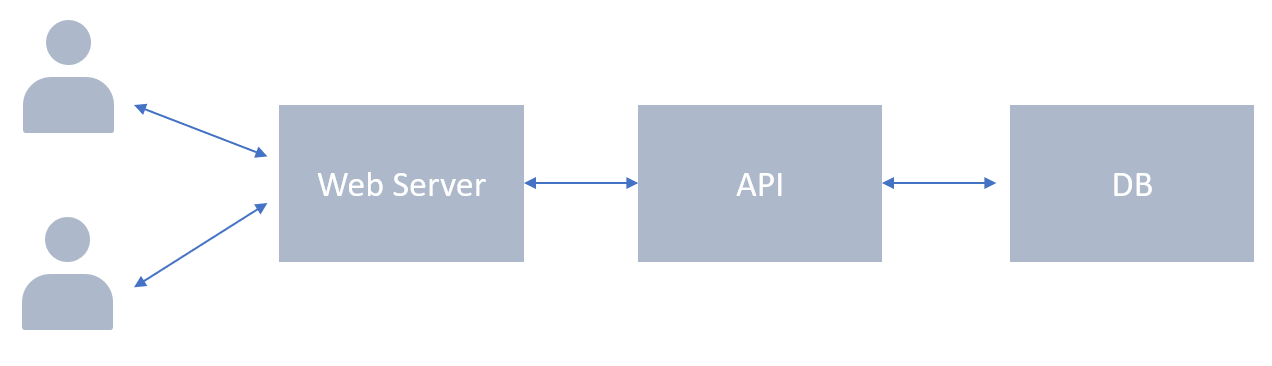
\includegraphics[width=\textwidth]{images/architektur.png}
  \caption[Architektur]{Architektur} 
  \label{Architektur}
\end{figure} 

Die in der Abbildung dargestellte Abbildung beschreibt, vereinfacht dargestellt, den Zusammenhang der einzelnen Komponenten. 
Ein Einblick in die konkrete Implementierung der Komponenten und Schnittstellen soll in den nächsten Abschnitten erfolgen. 

\subsection{Authentifizierung}

Authentifizierung sorgt dafür, dass ein Benutzer gegenüber einem System verifiziert werden kann.
Die Verifizierung erfolgt hierbei konventionell mit Wissen, also Benutzername und Passwort.
Nach dem Übertragen der Benutzerdaten wird von der API ein Token zurückgeschickt.
Ein, mittels Token gestützes Authentifizierungsverfahren, bietet die Möglichkeit den Benutzer mittels 
der API mit einem temporären Token anstatt seiner Benutzerdaten zu authentifizieren. 
Für das Beispiel wurden hierfür JSON Web Tokens \cite{JWT} eingesetzt. 
Der Vorteil von JSON Web Tokens liegt darin, dass der Token zusätzliche eingebettete Informationen
enthalten kann. 
Die zusätzlichen Informationen können von dem Client genutzt werden um dem Benutzer 
nur Zugriff auf einen Teil der Anwendung zu gewähren. 
Hier ist eine Grafik die, die Kommunikation der Komponenten anschaulich darstellt.

\begin{figure}
  \centering
  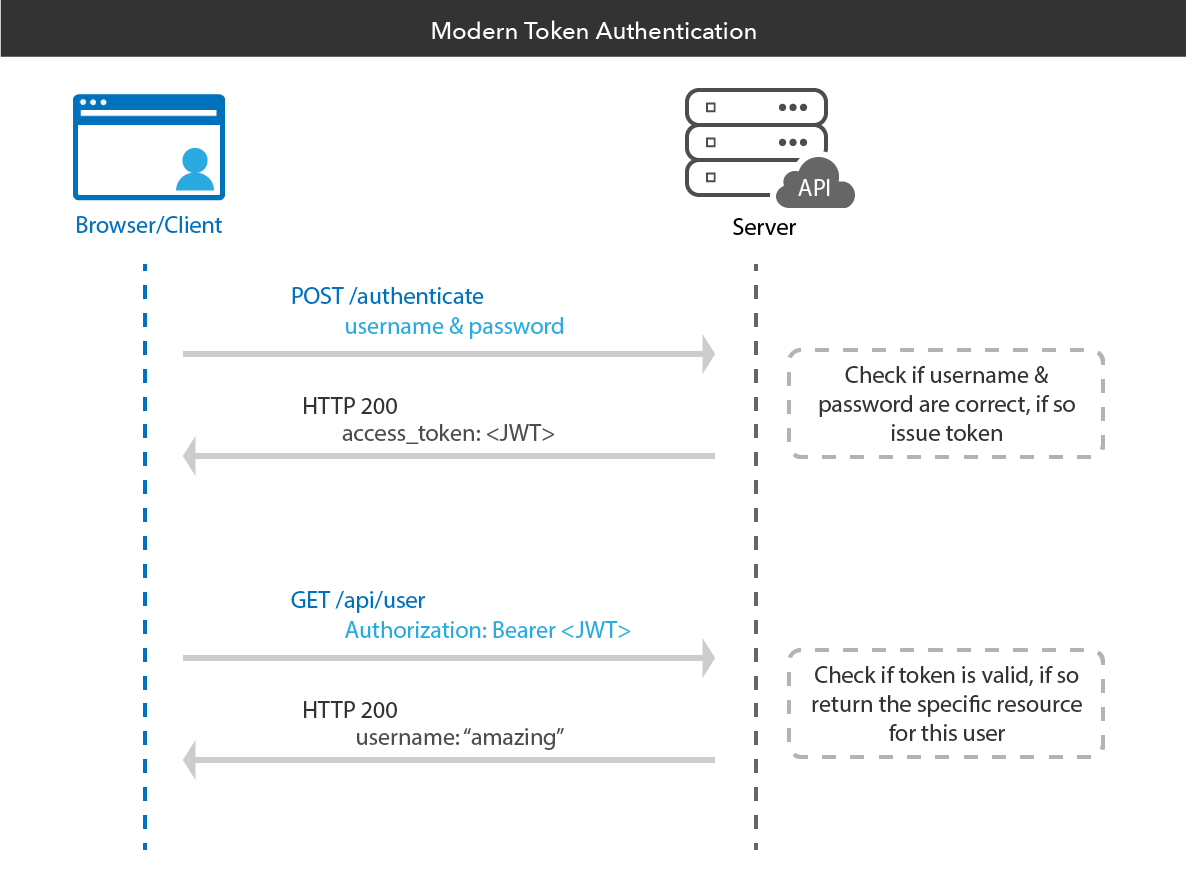
\includegraphics[width=\textwidth]{images/token-auth.png}
  \caption[Token Authentification]{Token Authentification} 
  \label{token-auth}
  \cite{OktaJWTAuth}
\end{figure} 

Nachdem der Benutzer seine Daten in die Entsprechenden Felder eingegeben hat, werden die Daten 
mittels HTTP-POST an die API übertragen.

\begin{verbatim}
onSubmit = (e) => {
  axios
    .post("http://api.domain.com:5001/register", {
      username: this.state.username,
      password: this.state.password,
      mail: this.state.mail,
    })
    .then((auth) => {
      if (auth) {
        localStorage.setItem("key", auth.data.key);
      }
    }
}
\end{verbatim}

Werden die korrekten Anmeldedaten eingegeben bzw. registriert sich der Benutzer an der 
Anwendung, sendet der Server als Antwort einen Token. 
Der JWT-Token besteht aus drei wichtigen Informationen: Header, Payload und Verify Signature.
Die drei Informationen wurden auf dem Server codiert und als Zeichenkette zurückgegeben. 
Die Zeichenkette wird in den localStorage des Client gespeichert. Wird anschließend eine 
geschützte Ressource von dem Server angefragt wird der Token aus dem localStorage geholt 
und in den Header der Anfrage geschrieben.
Auf der API durchläuft die Anfrage mehrere Middlewares. 
Bei geschützten Ressourcen wird wie in der folgenden Darstellung eine Middleware 
zwischengeschaltet. 

\begin{verbatim}
router.get("/", allowCustomer, async(req, res, next) => {
  res.json(item);
});
\end{verbatim}

Die Middleware gibt die Anfrage an die nachfolgende Middleware weiter wenn der im Header enthaltene 
Token korrekt ist. Ist der Token nicht korrekt gelangt die Anfrage erst gar nicht an die nächste Funktion die,
die eigentlichen Inhalte zurückgeben würde. 
Die API sendet dem Client den entsprechenden Status Code und dieser kann die Antwort bspw. in Form 
einer Fehler-Nachricht an den Benutzer weiter geben. 

\subsection{Vertraulichkeit und Zugriffssteuerung}

Der Sicherheitdienst der Vertraulichkeit macht bestimmte Teile der Anwendung nur für einen Teil der Benutzer sichtbar. 
Das Beispiel verfügt über eine Rollenbasierte Zugriffssteuerung. 
Rollen die ein Benutzer annehmen kann sind: 
\begin{itemize}
  \item Administrator
  \item Customer
  \item Guest
\end{itemize}

Ein Benutzer der über die Rolle "Guest" verfügt soll lediglich in die Lage sein die Items auf der Website anzuschauen. 
Ist ein Benutzer angemeldet, verfügt dieser über die Rolle "Customer" und darf Artikel einkaufen. 
Ein Benutzer mit der Rolle Administrator kann auf zusätzlich zu den Anderen Seiten, auf eine spezielle Administrator Seite zugreifen, die ihm eine Übersicht über 
alle Benutzerdaten liefert. 
Den Zugriff kann man mittels der folgenden Grafik veranschaulichen:

\begin{figure}
  \centering
  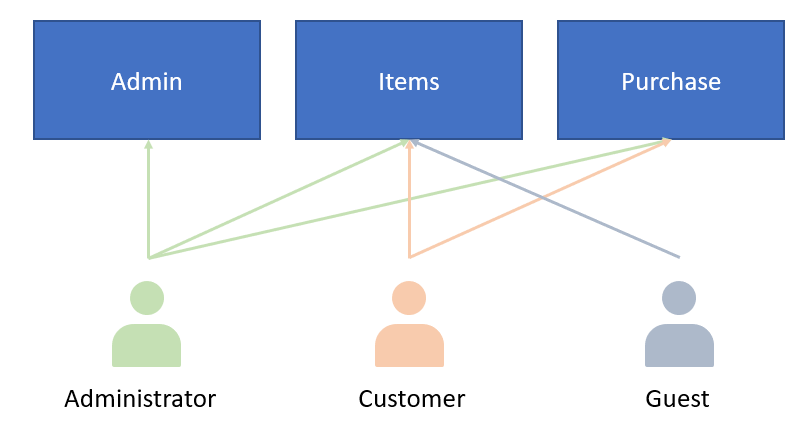
\includegraphics[width=\textwidth]{images/access.png}
  \caption[Zugriffsbeschränkunen]{Zugriffsbeschränkunen} 
  \label{access-desc}
\end{figure} 

Um eine solche Zugriffsunterscheidung durchführen zu können, wird auf der API der Zugriff durch Middlewares ausgeschlossen. 
Das Verfahren wird mithilfe von verschiedenen Middlewares implementiert. Das Verfahren wurde im vorherigen Abschnitt 
bereits genauer erläutert. 
Mit der Implementierung von Middlewares sind bestimmte Ressourcen auf der Oberfläche nur einem Teil der Benutzer zugänglich. 
Allerdings werden bspw. Verweise auf gesperrte Ressourcen weiterhin angezeigt. 
Die Client-Applikation muss über die Information verfügen, wer momentan die Anwendung bedient und über welche Berechtigungen er verfügt. 
Eine Möglichkeit wäre den Json Web Token, der während einer Session im Local Storage gespeichert wird, zu decodieren und anschließend 
mithilfe der Berechtigung der Payload nur ausgewählte Ressourcen anzuzeigen. 
Zur Decodierung eines JWT ist das Wissen über das Secret notwendig mit dessen Hilfe der Token erstellt wurde. 
Erhält der Benutzer das Secret um auf Client-Seite zu entschlüsseln bietet das ein Gefahrenpotential. 
Der Benutzer wäre in der Lage eigene Tokens zu erstellen mit denen er über erweiterte Rechte verfügt. 
Die Encodierung der Tokens darf aus diesem Grund nur auf der API erfolgen. 
Um eine sichere Entschlüsselung der Tokens durchzuführen wird dieser von der Client-Applikation an die API 
gesendet. Die API entschlüsselt die Nachricht und sendet die Payload dem Benutzer zurück. 
Da bei der Antwort der API wichtige Anmeldedaten in Textform übertragen werden muss die Verbindung vor Man-In-The-Middle Attacken geschützt werden. 
Die Verbindung zwischen Client und Server wird aus diesem Grund mittels HTTPS Verschlüsselt. 
Für die Implementierung der Anwendung wird vor die Komponenten ein NGINX Reverse Proxy eingesetzt. 

\begin{figure}
  \centering
  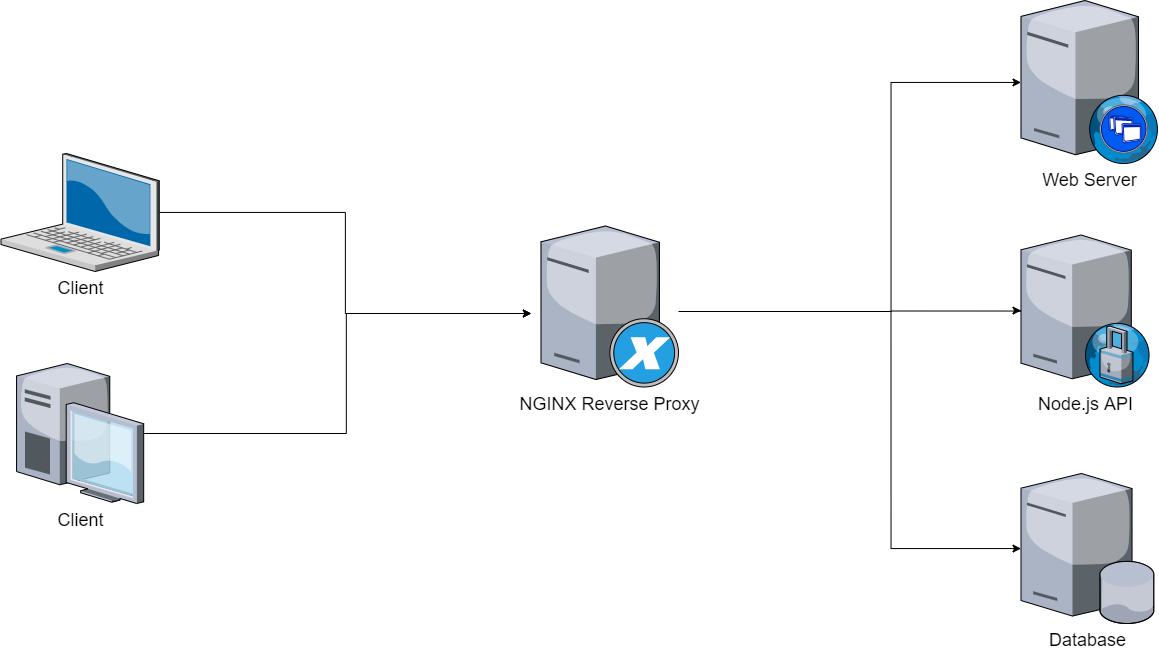
\includegraphics[width=\textwidth]{images/reversep.png}
  \caption[Reverse Proxy]{Reverse Proxy} 
  \label{Reverse-proxy}
\end{figure} 

Alle Anfragen die auf eine der Komponenten treffen werden über den Reverse Proxy verteilt. Die Verschlüsselung wird 
in dem Reverse Proxy vorgenommen. 

\begin{verbatim}
  server {
    listen 80;
    listen [::]:80;

    server_name api.domain.com;

    location / {
                proxy_pass http://192.168.0.2:5000;
    }
  }
\end{verbatim}

Bei der Konfiguration des Reverse Proxy muss der Eingangsport und die Domain angegeben werden, über die eine eingehende Anfrage auf den Reverse Proxy trifft. 
Mittels des "location" Bocks wird angegeben auf welchen Server die Anfrage umgeleitet wird. 
Durch Zertifikations Tools wie Certbot können direkt an dieser Stelle notwendige Informationen für eine HTTPS Verbindung festgelegt werden. 
\\\\
Das Sicherheitsziel der Zugriffsteuerung und der Vertraulichkeit sind damit weitestgehend abgedeckt. 
Da in der Anwendung mit einer Datenbank gearbeitet wird, ist bei der Persistierung von Benutzerdaten und besonders Passwörtern ein weiterer Aspekt zu beachten. 
In der Datenbank dürfen Passwörter nicht in Klartext abgelegt werden. 
Bevor die Daten initial in der Datenbank abgelegt und gespeichert werden muss mittels Hash Algorithmus noch eine Verfremdung erfolgen. 
Im Node.js Umfeld wird dafür Typischerweise das Tool "BCrypt" benutzt. Mithilfe von BCrypt kann man Passwörter Hashen und zum Späteren Zeitpunkt 
mit einem Klartextwort vergleichen um eine Authentifizierung durchzuführen. 
Ein Benutzerobjekt wird in der Datenbank folgendermaßen gespeichert: 

\begin{verbatim}
{
  "TestBenutzerName":
      {
          "username":"TestBenutzerName",
          "password":"$2b$05$/6mQI7c.5BtWkpYwsTGfReLR7iWZAA9.psfgVSxTiDW40AJIhOAbS",
          "mail":"test.benutzer@email.com",
          "role":2
      }
}
\end{verbatim}



\subsection{Integrität}
\subsection{Nicht-Anfechtbarkeit}
\subsection{Verfügbarkeit}

\section{Fazit}


%% \bibliography{lni-paper-example-de.tex} ist hier nicht erlaubt: biblatex erwartet dies bei der Preambel
%% Starten Sie "biber paper", um eine Biliographie zu erzeugen.
\printbibliography

\end{document}
